%-----------------------------------------------------------------------------
%	PACKAGES AND DOCUMENT CONFIGURATIONS
%-----------------------------------------------------------------------------

\documentclass{article}

\usepackage{graphicx} % Required for the inclusion of images
\usepackage{natbib} % Required to change bibliography style to APA
\usepackage{amsmath} % Required for some math elements
\usepackage{amssymb}
\usepackage{grffile}
\usepackage[export]{adjustbox}
\usepackage{subcaption}
\usepackage{float}
\usepackage{listings}
\usepackage[margin=1.0in]{geometry}
\usepackage{tikz}
\usepackage{enumitem}
\usepackage{scrextend}
\usepackage{siunitx}
\usepackage{minted}

\usetikzlibrary{shapes.geometric, arrows}
\tikzstyle{startstop} = [rectangle, rounded corners, minimum width=1cm, minimum height=1cm,text centered, draw=black, fill=white!30]
\tikzstyle{process} = [rectangle, minimum width=1cm, minimum height=1cm, text centered, draw=black, fill=white!30]
\tikzstyle{arrow} = [thick,->,>=stealth]

\setlength\parindent{0pt} % Removes all indentation from paragraphs

%-----------------------------------------------------------------------------
%	DOCUMENT INFORMATION
%-----------------------------------------------------------------------------

\title{ECE 547 Fall 2016 Homework 2} % Title

\author{Yang \textsc{Wang}}  % Author name

\date{\today} % Date for the report

\renewcommand{\theenumi}{\alph{enumi}} % use letters for list items

\begin{document}

\maketitle % Insert the title, author and date

%-----------------------------------------------------------------------------
%	Problem 1
%-----------------------------------------------------------------------------

\section*{Probability Review Problems}
	\subsection*{Problem 1}
		\begin{enumerate}
			\item Since $X$ and $Y$ have identical distributions,
				\begin{gather*}
					P(\left\{X \in A\right\}) = P(\left\{Y \in A\right\}), A \in \mathbb{R} \\
					\implies X = Y
				\end{gather*}
				Therefore, the statement is \textbf{true}.
			\item Since $X$ and $Y$ have identical distributions,
				let $F(t) = P(\left\{X \leq t\right\}) = P(\left\{Y \leq t\right\})$,
				\begin{gather*}
					\implies E[X] = E[Y] = \int_{\mathbb{R}}^{}t \cdot dF(t)
				\end{gather*}
				Therefore, the statement is \textbf{true}.
			\item The statement is \textbf{false}.
				
				Say we have r.v.'s $X$, $Y$, and
				$Z$. $X$ is independent from $Y$. $Y$ is independent from $Z$ and $X = Z$.
				Then, $X$ is \textbf{not} independent from $Z$.
		\end{enumerate}

	\subsection*{Problem 2}
		\begin{enumerate}
			\item We know $X$ is a non-negative r.v. with distribution $F$, using the
				definition of expected value of a r.v.,
				\begin{align*}
					E[X] &= \int_{0}^{\infty} xf_{X}(x)dx \\
					&= \int_{0}^{\infty} xdF_{X}(x) \\
					&= -\int_{0}^{\infty} xd\bar{F}_X(x) \\
				\end{align*}
				Using integration by parts,
				let $u = x$, $du = dx$, $dv = d\bar{F}_{X}(x)$, then $v = \bar{F}_{X}(x)$,
				\begin{align*}
					E[X] &= -x\bar{F}_{X}(x) \bigg|_{0}^{\infty} + \int_{0}^{\infty}\bar{F}_{X}(x)dx \\
					&= -x\bar{F}_{X}(x) \bigg|_{0}^{\infty} + \int_{0}^{\infty}(1 - F_{X}(x))dx \\
					&= 0 + \int_{0}^{\infty}(1 - F_{X}(x))dx \\
					&= \int_{0}^{\infty}P(\left\{ X > x \right\})dx
				\end{align*}
			\item From the definition of the expected value of a r.v.,
				\begin{align*}
					E[X^n] &= \int_{0}^{\infty} x^nf_{X}(x)dx \\
					&= -\int_{0}^{\infty} x^nd\bar{F}_X(x)
				\end{align*}
				Using the same integration by parts method, we can get,
				\begin{align*}
					E[X] &= -x^n\bar{F}_{X}(x) \bigg|_{0}^{\infty} + \int_{0}^{\infty}nx^{n-1}\bar{F}_{X}(x)dx \\
					&= -x^n\bar{F}_{X}(x) \bigg|_{0}^{\infty} + \int_{0}^{\infty}nx^{n-1}(1 - F_{X}(x))dx \\
					&= 0 + \int_{0}^{\infty}nx^{n-1}(1 - F_{X}(x))dx \\
					&= \int_{0}^{\infty}nx^{n-1}P(\left\{ X > x \right\})dx
				\end{align*}
		\end{enumerate}

	\subsection*{Problem 3}
		\begin{enumerate}
			\item From $E[E[X \mid Y]]$, we can have,
				\begin{align*}
					E[E[X \mid Y]] &= \int_{-\infty}^{\infty} E[X \mid Y] dF_{Y}(y) \\
					&= \int_{-\infty}^{\infty}\int_{-\infty}^{\infty}x dF_{X}(x \mid y)dF_{Y}(y) \\
					&= \int_{-\infty}^{\infty}\int_{-\infty}^{\infty}x \frac{dF_{XY}(x,y)}{dF_{Y}(y)} dF_{Y}(y) \\
					&= \int_{-\infty}^{\infty}\int_{-\infty}^{\infty}x dF_{XY}(x,y) \\
					&= \int_{-\infty}^{\infty}x dF_{X}(x) = E[X]
				\end{align*}
			\item From the definition of joint expectation,
				\begin{align*}
					E[XY] = \iint_{}xyf_{XY}(x,y) \,dx\,dy
				\end{align*}
				Since $X$ and $Y$ are statistically independent, hence,
				\begin{align*}
					E[XY] &= \iint_{}xyf_{XY}(x,y) \,dx\,dy \\
					&= \int_{}^{}xf_X{x}dx \int_{}^{}yf_Y{y}dy \\
					&= E[X]E[Y]
				\end{align*}
				Therefore, $X$ and $Y$ are uncorrelated. The converse of this statement is
				\textbf{not true}. A counterexample:
				\begin{align*}
					X & \sim \mathrm{\textit{U}}(-1,1) \\
					Y &= X^2
				\end{align*}
				E[XY] = 0 but $X$ and $Y$ are dependent.
			\item We know $\Psi_{Z}(t) = E[e^{tZ}]$,
				\begin{align*}
					\Psi_{X+Y}(t) = E[e^{t(X+Y)}] = E[e^{tX}e^{tY}]
				\end{align*}
				We know $X$ and $Y$ are statistically independent, therefore,
				\begin{align*}
					E[e^{tX}e^{tY}] &= E[e^{tX}]E[e^{tY}] \\
					&= \Psi_{X}(t)\Psi_{Y}(t) \\
					\implies \Psi_{X+Y}(t) &= \Psi_{X}(t)\Psi_{Y}(t)
				\end{align*}
				From the moment theorem, we know,
				\begin{equation}
					E[X^n] = \frac{d^n\Psi_{X}(t)}{dt^n} = \Psi_{X}^{(n)}(0)
					\label{eq:1}
				\end{equation}
				Using equation \ref{eq:1}, for $E[X]$, we can see,
				\begin{align*}
					E[X] &= \frac{d\Psi_{X}(t)}{dt} = \frac{n}{\lambda}\left(\frac{\lambda}{\lambda-t}\right)^{n+1} \bigg|_{t=0} \\
					&= \frac{n}{\lambda}
				\end{align*}
				We know Var$[X] = E[X^2] - \left(E[X]\right)^2$, then,
				\begin{align*}
					\mathrm{Var}[X] &= \frac{d^2\Psi_{X}(t)}{dt^2} - \left(\frac{n}{\lambda}\right)^2 \\
					&= \frac{n(n+1)\left(\frac{\lambda}{\lambda-t}\right)^n}{\left(\lambda-t\right)^2} - \left(\frac{n}{\lambda}\right)^2 \bigg|_{t=0} \\
					&= \frac{n(n+1)}{\lambda^2} - \frac{n^2}{\lambda^2} \\
					&= \frac{n}{\lambda^2}
				\end{align*}
			\item We need to prove $\mathrm{Var}[X] = E[X^2] - (E[X])^2 = E[\mathrm{Var}(X \mid Y)] + \mathrm{Var}(E[X \mid Y])$.

				From $\mathrm{Var}[X] = E[X^2] - (E[X])^2$, we can have,
				\begin{align*}
					E[X^2] - (E[X])^2 &= E[E[X^2 \mid Y]] - (E[E[X \mid Y]])^2 \\
					&= E[\mathrm{Var}[X \mid Y] + (E[X \mid Y])^2] - (E[E[X \mid Y]])^2 \\
					&= E[\mathrm{Var}[X \mid Y]] + (E[E[X \mid Y]^2] - (E[E[X \mid Y]])^2) \\
					&= E[\mathrm{Var}[X \mid Y]] + \mathrm{Var}(E[X \mid Y])
				\end{align*}

				From $E[\mathrm{Var}(X \mid Y)]$, we have,
				\begin{align*}
					E[\mathrm{Var}(X \mid Y)] &= E[E[(X - E[X \mid Y])^2 \mid Y]] \\
					&= E[(X - E[X \mid Y])^2] \\
					&= E[X^2 -2X \cdot E[X \mid Y] + E^2[X \mid Y]] \\
					&= E[X^2] - 2E[X \cdot E[X \mid Y]] + E[E^2[X \mid Y]]
				\end{align*}
				From $\mathrm{Var}(E[X \mid Y])$, we have,
				\begin{align*}
					\mathrm{Var}(E[X \mid Y]) &= E[E^2[X \mid Y]] - (E[E[X \mid Y]])^2 \\
					&= E[E^2[X \mid Y]] - (E[X])^2
				\end{align*}
				Then $\mathrm{Var}(X)$ becomes,
				\begin{align*}
					\mathrm{Var}(X) &= E[X^2] - 2E[X \cdot E[X \mid Y]] + E[E^2[X \mid Y]] + E[E^2[X \mid Y]] - (E[X])^2 \\
					&= E[X^2] - 2E[X \cdot E[X \mid Y]] + 2E[E^2[X \mid Y]] - (E[X])^2 \\
					&= E[X^2] - (E[X])^2 \\
					&= \mathrm{Var}(X)
				\end{align*}
		\end{enumerate}

	\subsection*{Problem 4}
		\begin{enumerate}
			\item The moment generating function of $Y$ is,
				\begin{align*}
					\Psi_{Y}(t) = E[e^{tY}] = E[e^{t \sum_{i=1}^{N}X_{i}}]
				\end{align*}
				Given that $X_{i}$'s are independent, hence,
				\begin{align*}
					\Psi_{Y}(t) &= E[e^{tX_{1}}]E[e^{tX_{2}}]E[e^{tX_{3}}] \ldots E[e^{tX_{N}}] \\
					&= E[E[e^{t \sum_{i=1}^{N}X_{i}} \mid N]] \\
					&= E[\Psi_{X}(t)^N]
				\end{align*}
			\item For finding $E(Y)$ and x$\mathrm{Var}(Y)$, we can first differentiate $\Psi_{Y}(t)$,
				\begin{align*}
					E[Y] &= \Psi'_{Y}(t) \bigg|_{t=0} \\
					&= E[N \Psi_{X}(t)^{N-1} \Psi'_{X}(t)] \bigg|_{t=0} \\
					&= E[N]E[X]
				\end{align*}
				Also,
				\begin{align*}
					E[Y^2] &= \Psi''_{Y}(t) \bigg|_{t=0} \\
					&= E[N(N-1)\Psi_{X}(t)^{N-2} \Psi'_{X}(t)^2 + N \Psi_{X}(t)^{N-1} \Psi''_{X}(t)] \bigg|_{t=0} \\
					&= E[N(N-1)E^2[X] + NE[X^2]]
				\end{align*}
				Hence,
				\begin{align*}
					\mathrm{Var}(Y) &= E[Y^2] - (E[Y])^2 = E[N(N-1)E^2[X] + NE[X^2]] - (E[N]E[X])^2 \\
					&= E[N(N-1)E^2[X]] + E[NE[X^2]] - E^2[N]E^2[X] \\
					&= E[N](E[N] - 1)E[E^2[X]] + E[N]E[E[X^2]] - E^2[N]E^2[X] \\
					&= E^2[N](E[E^2[X]] - E^2[X]) - E[N](E[E^2[X]] - E[E[X^2]]) \\
					&= E^2[N]\mathrm{Var}(E[X]) + E[N](E[\mathrm{Var}(X)])
				\end{align*}
		\end{enumerate}

	\subsection*{Problem 5}
		\begin{enumerate}
			\item
				\begin{align*}
					P\left(\left\{ \text{all five cards are seven} \right\}\right) = 0
				\end{align*}
			\item
				\begin{align*}
					P\left(\left\{ \text{at least one of the cards is a seven} \right\}\right) &= 1 - \frac{\binom{48}{5}}{\binom{52}{5}} = 0.341
				\end{align*}
			\item
				\begin{align*}
					P\left(\left\{ \text{none of the cards is a seven} \right\}\right) &= \frac{\binom{48}{5}}{\binom{52}{5}} = 0.659
				\end{align*}
			\item
				\begin{align*}
					P\left(\left\{ \text{two out of the five cards are sevens} \right\}\right) &= \frac{\binom{3}{2}\binom{48}{5}}{\binom{52}{5}} = 0.040
				\end{align*}
		\end{enumerate}

	\subsection*{Problem 6}
		We can obtain from the given cdf,
		\begin{align*}
			P(\left\{ X = k \right\}) &= \frac{n!}{k!(n-k)!} p^k (1-p)^{n-k} \\
			&= \frac{n(n-1)(n-2) \ldots (n-k+1)}{k!} p^k (1-p)^{n-k} \\
			&= \frac{np(n-1)p(n-2)p \ldots (n-k+1)p}{k!} (1-p)^{n-k} \\
		\end{align*}
		As $n \rightarrow \infty$ and $p \rightarrow 0$, $np \rightarrow \lambda$,
		we can obtain,
		\begin{align*}
			P(\left\{ X = k \right\}) &= \frac{\lambda^k}{k!} (1-p)^{n-k} \\
			&= \frac{\lambda^k}{k!} e^{-\lambda}
		\end{align*}
		Hence, we can say that the distribution of the r.v. $X$ converges to that of
		a Poisson r.v. with mean $\lambda$.

\section*{Simulation-Based Experiments}
	\subsection*{Problem 7}
	%TODO
	\subsection*{Problem 8}
		\begin{figure}[!hbt]
			\centering
			\begin{subfigure}[!hbt]{0.45\linewidth}
				\centering
				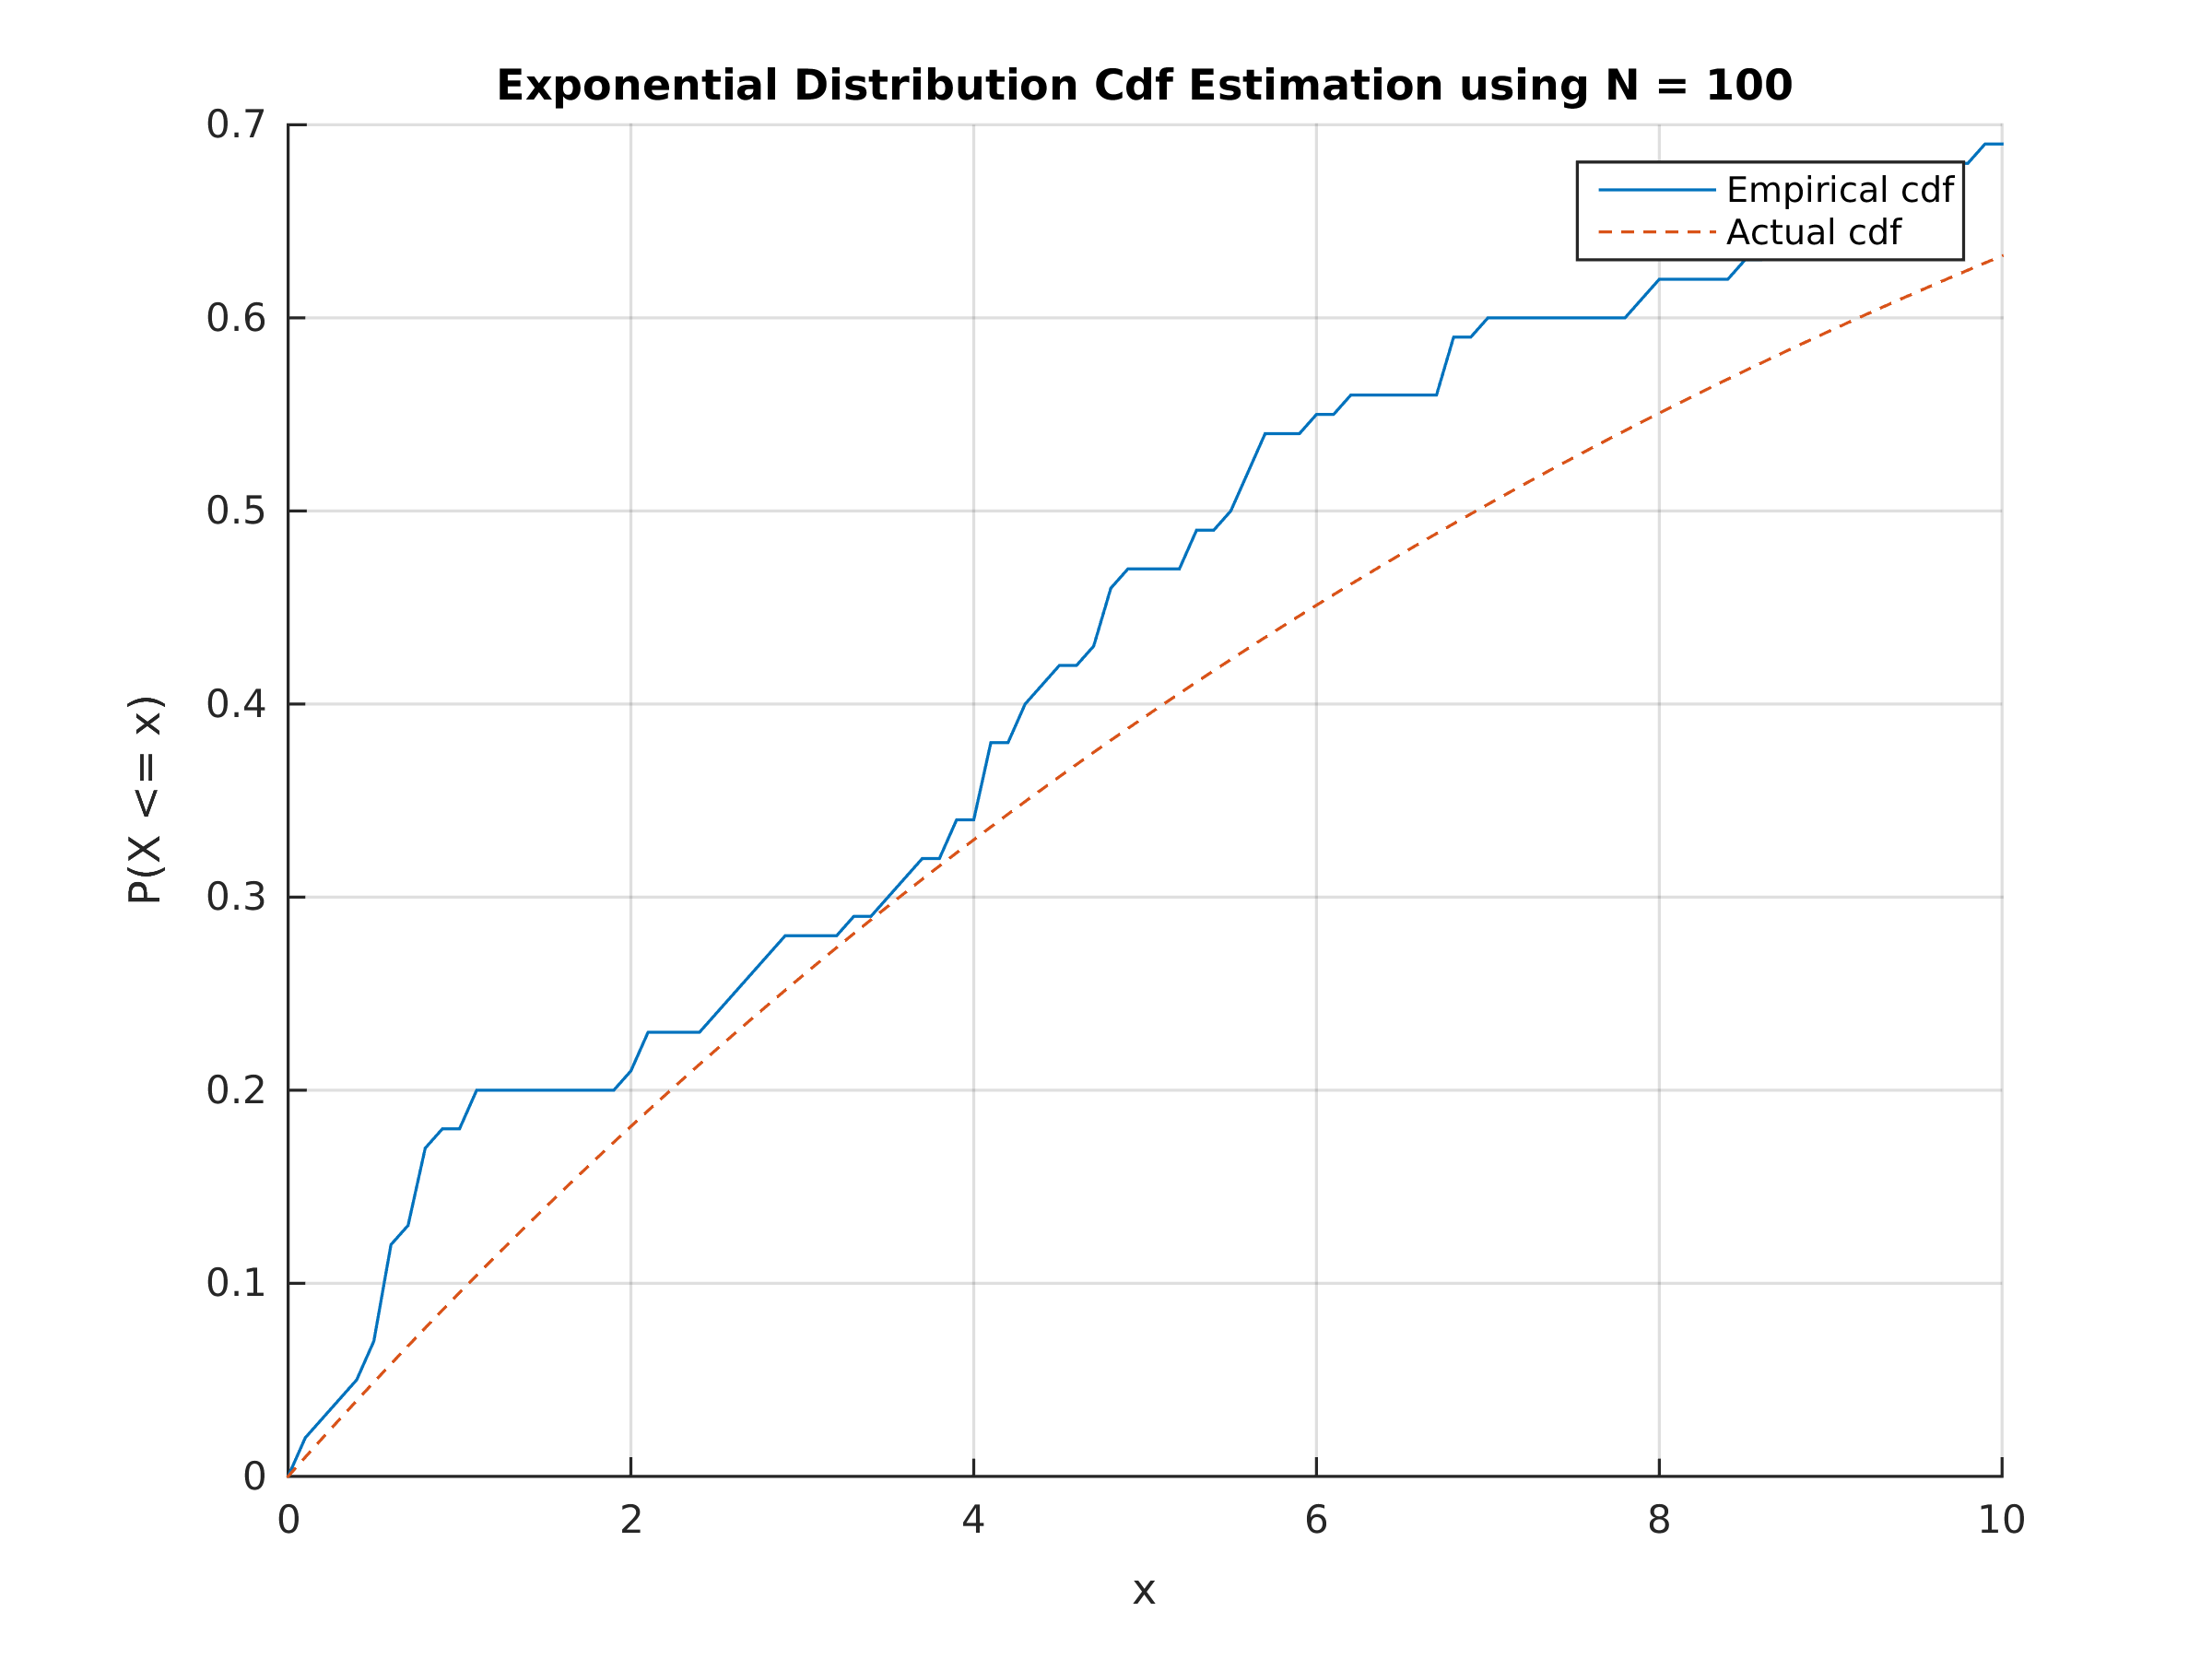
\includegraphics[width=1\linewidth]{hw2_8_exp_n100.png}
				\caption{Cdf using $N = 100$.}
			\end{subfigure}
			\begin{subfigure}[!hbt]{0.45\linewidth}
				\centering
				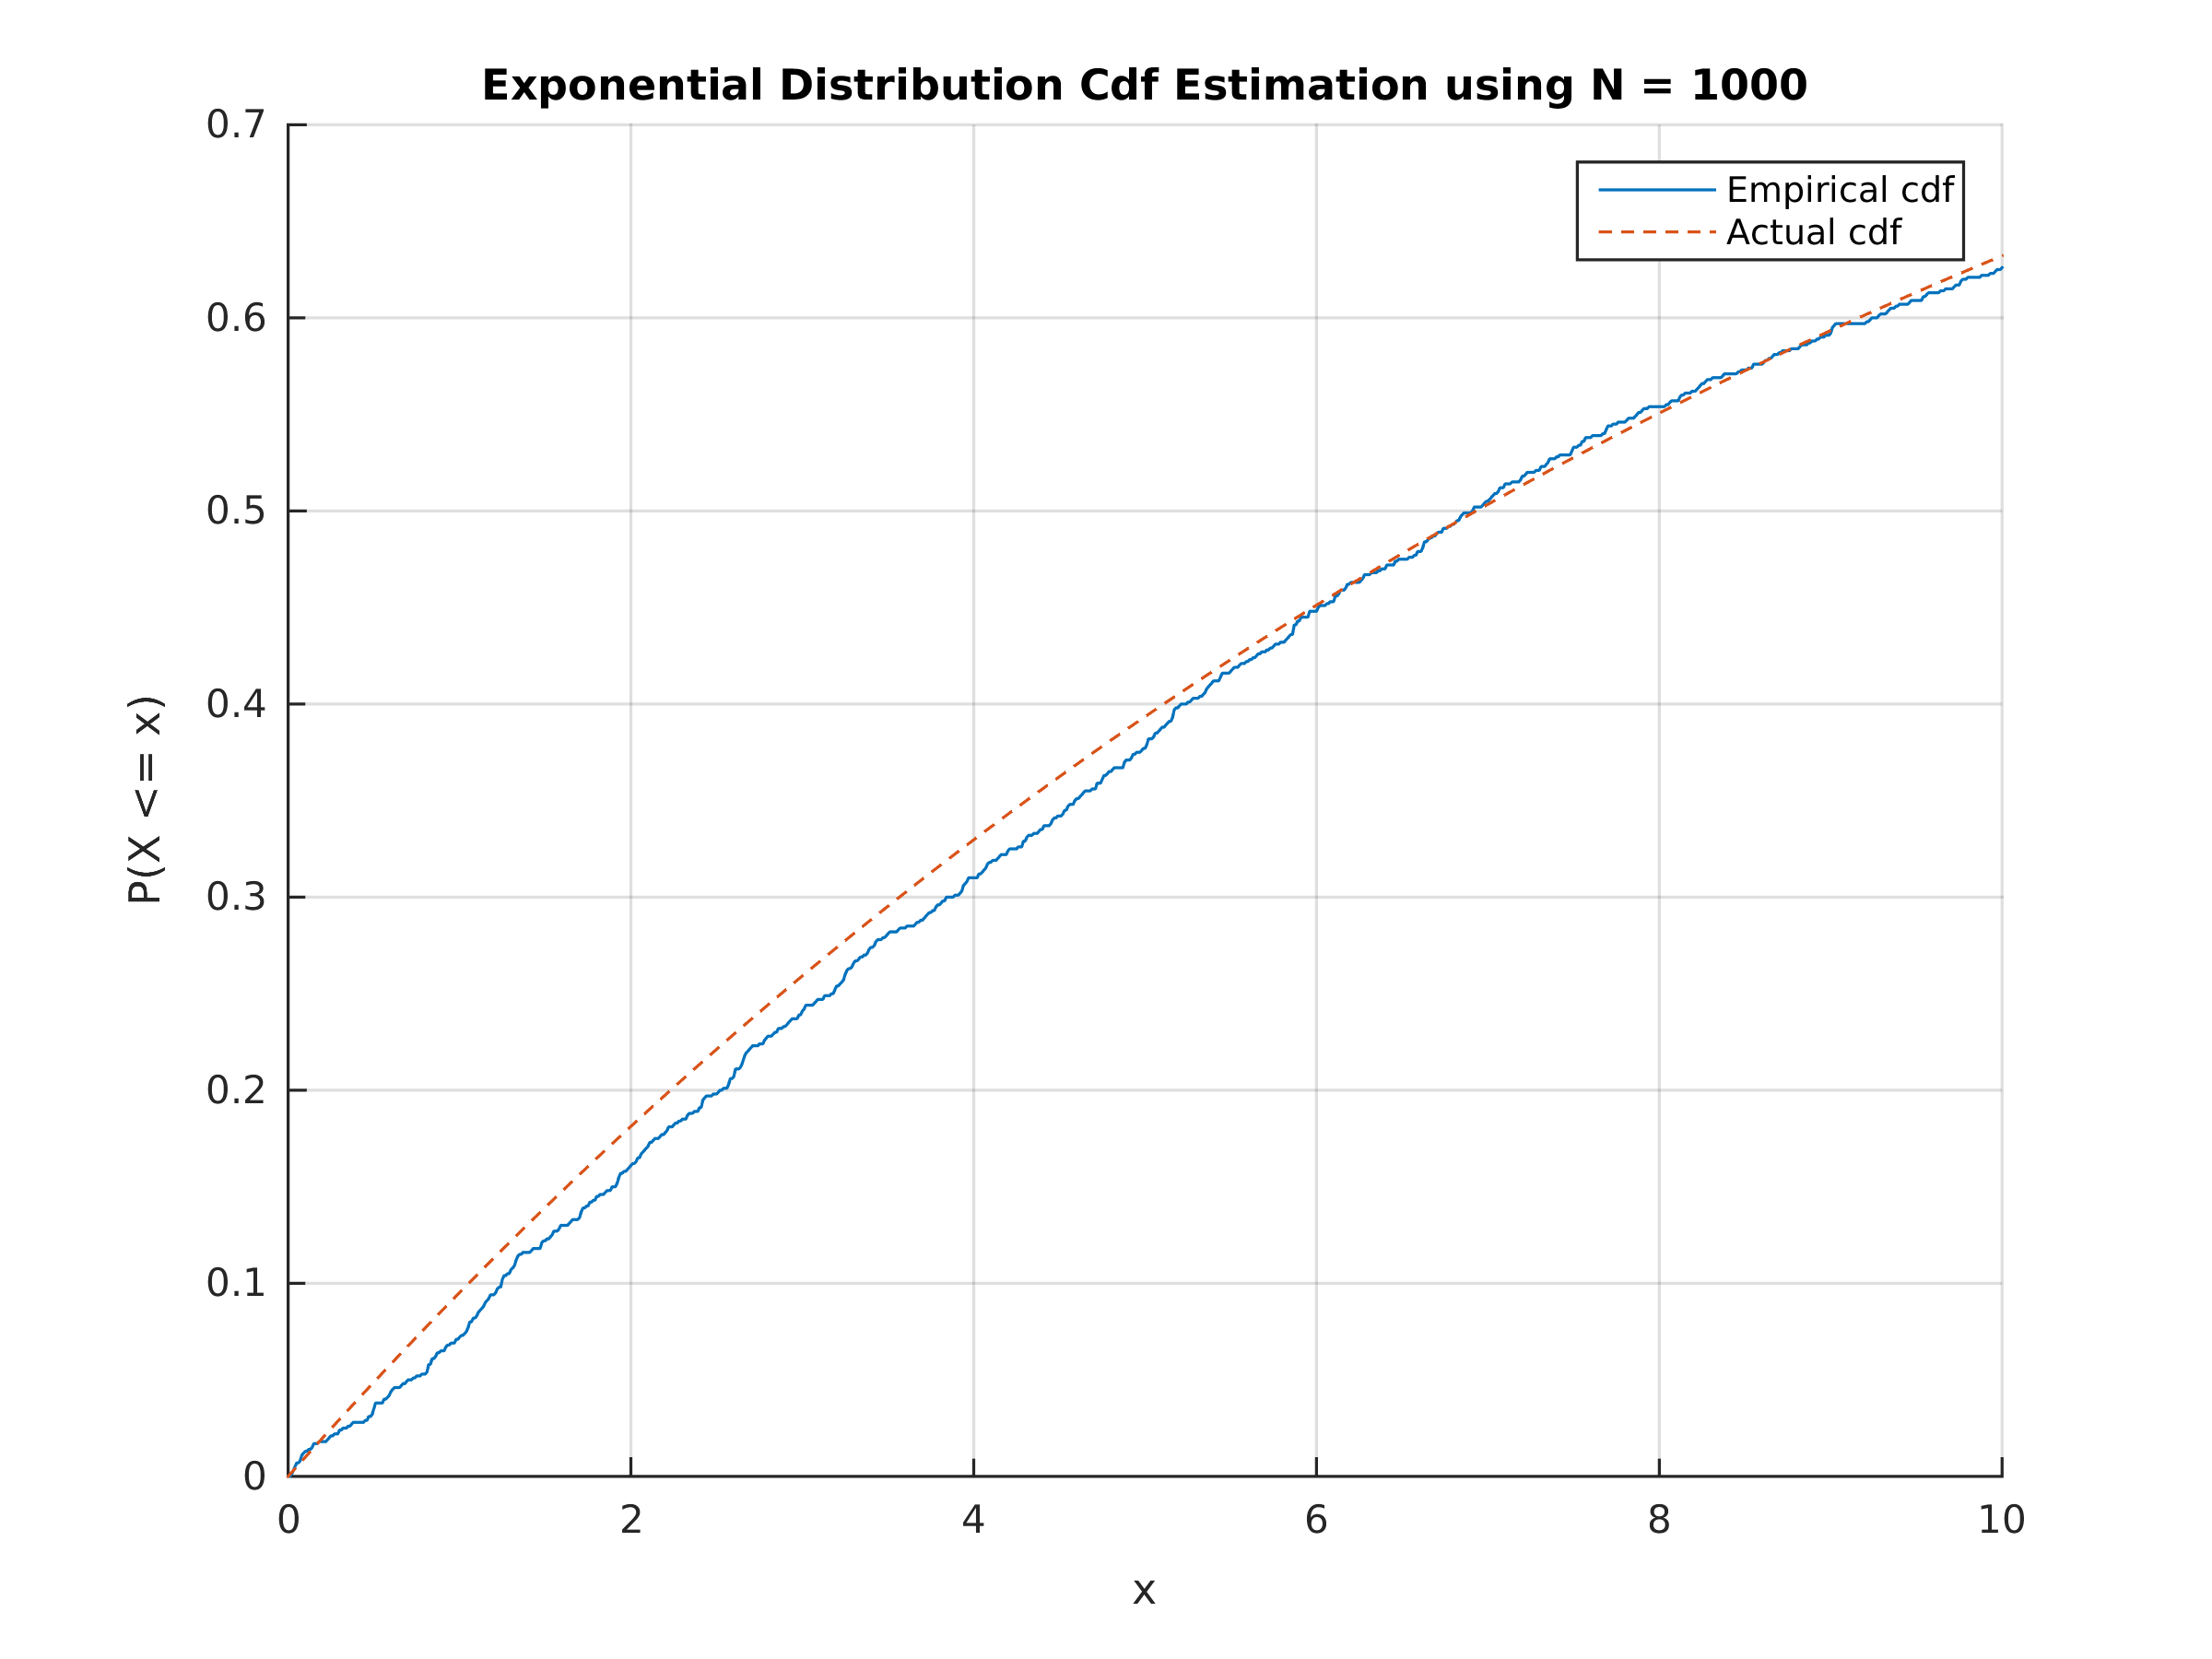
\includegraphics[width=1\linewidth]{hw2_8_exp_n1000.png}
				\caption{Cdf using $N = 1000$.}
			\end{subfigure}
			\caption{The cdf plots of exponential random variable $X$.}
		\end{figure}
		When $N = 100$, the cdf follows the trend of the actual exponential
		distribution but does not fit entirely. When using 1000 samples, the cdf
		fits nicely. $E[X] = ???$.
		\begin{figure}[!hbt]
			\centering
			\begin{subfigure}[!hbt]{0.45\linewidth}
				\centering
				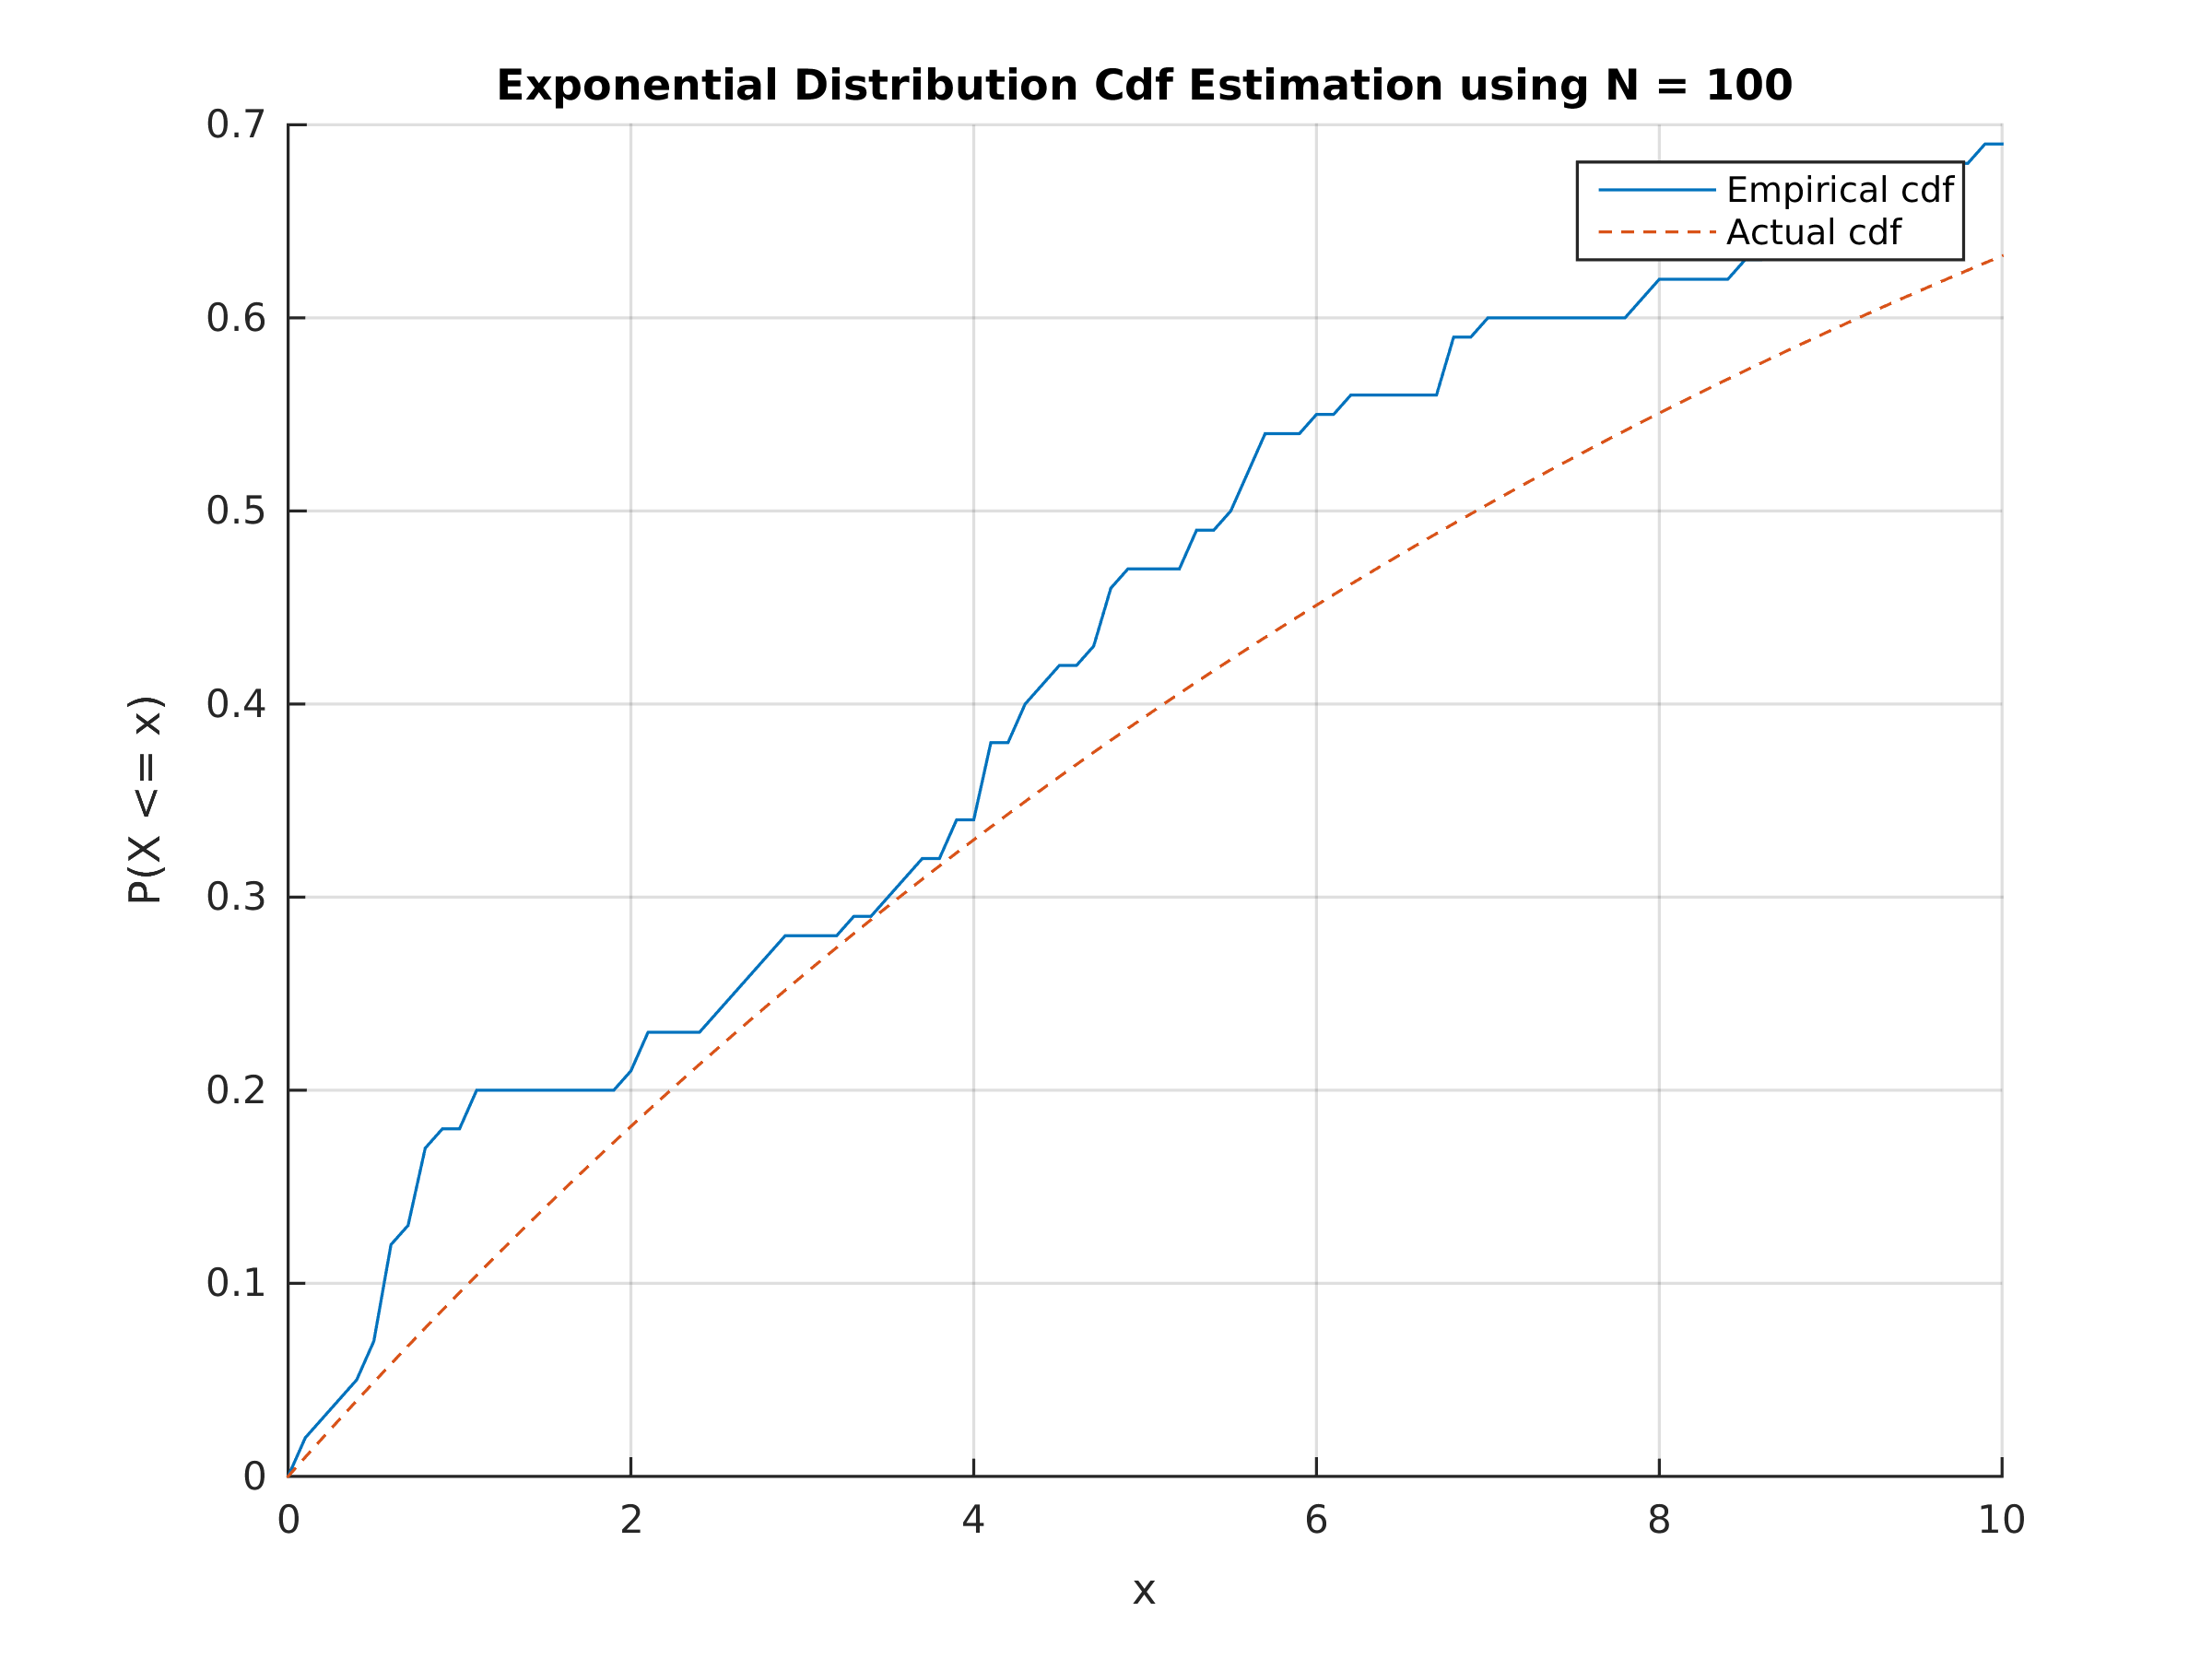
\includegraphics[width=1\linewidth]{hw2_8_exp_n100.png}
				\caption{Cdf using $N = 100$.}
			\end{subfigure}
			\begin{subfigure}[!hbt]{0.45\linewidth}
				\centering
				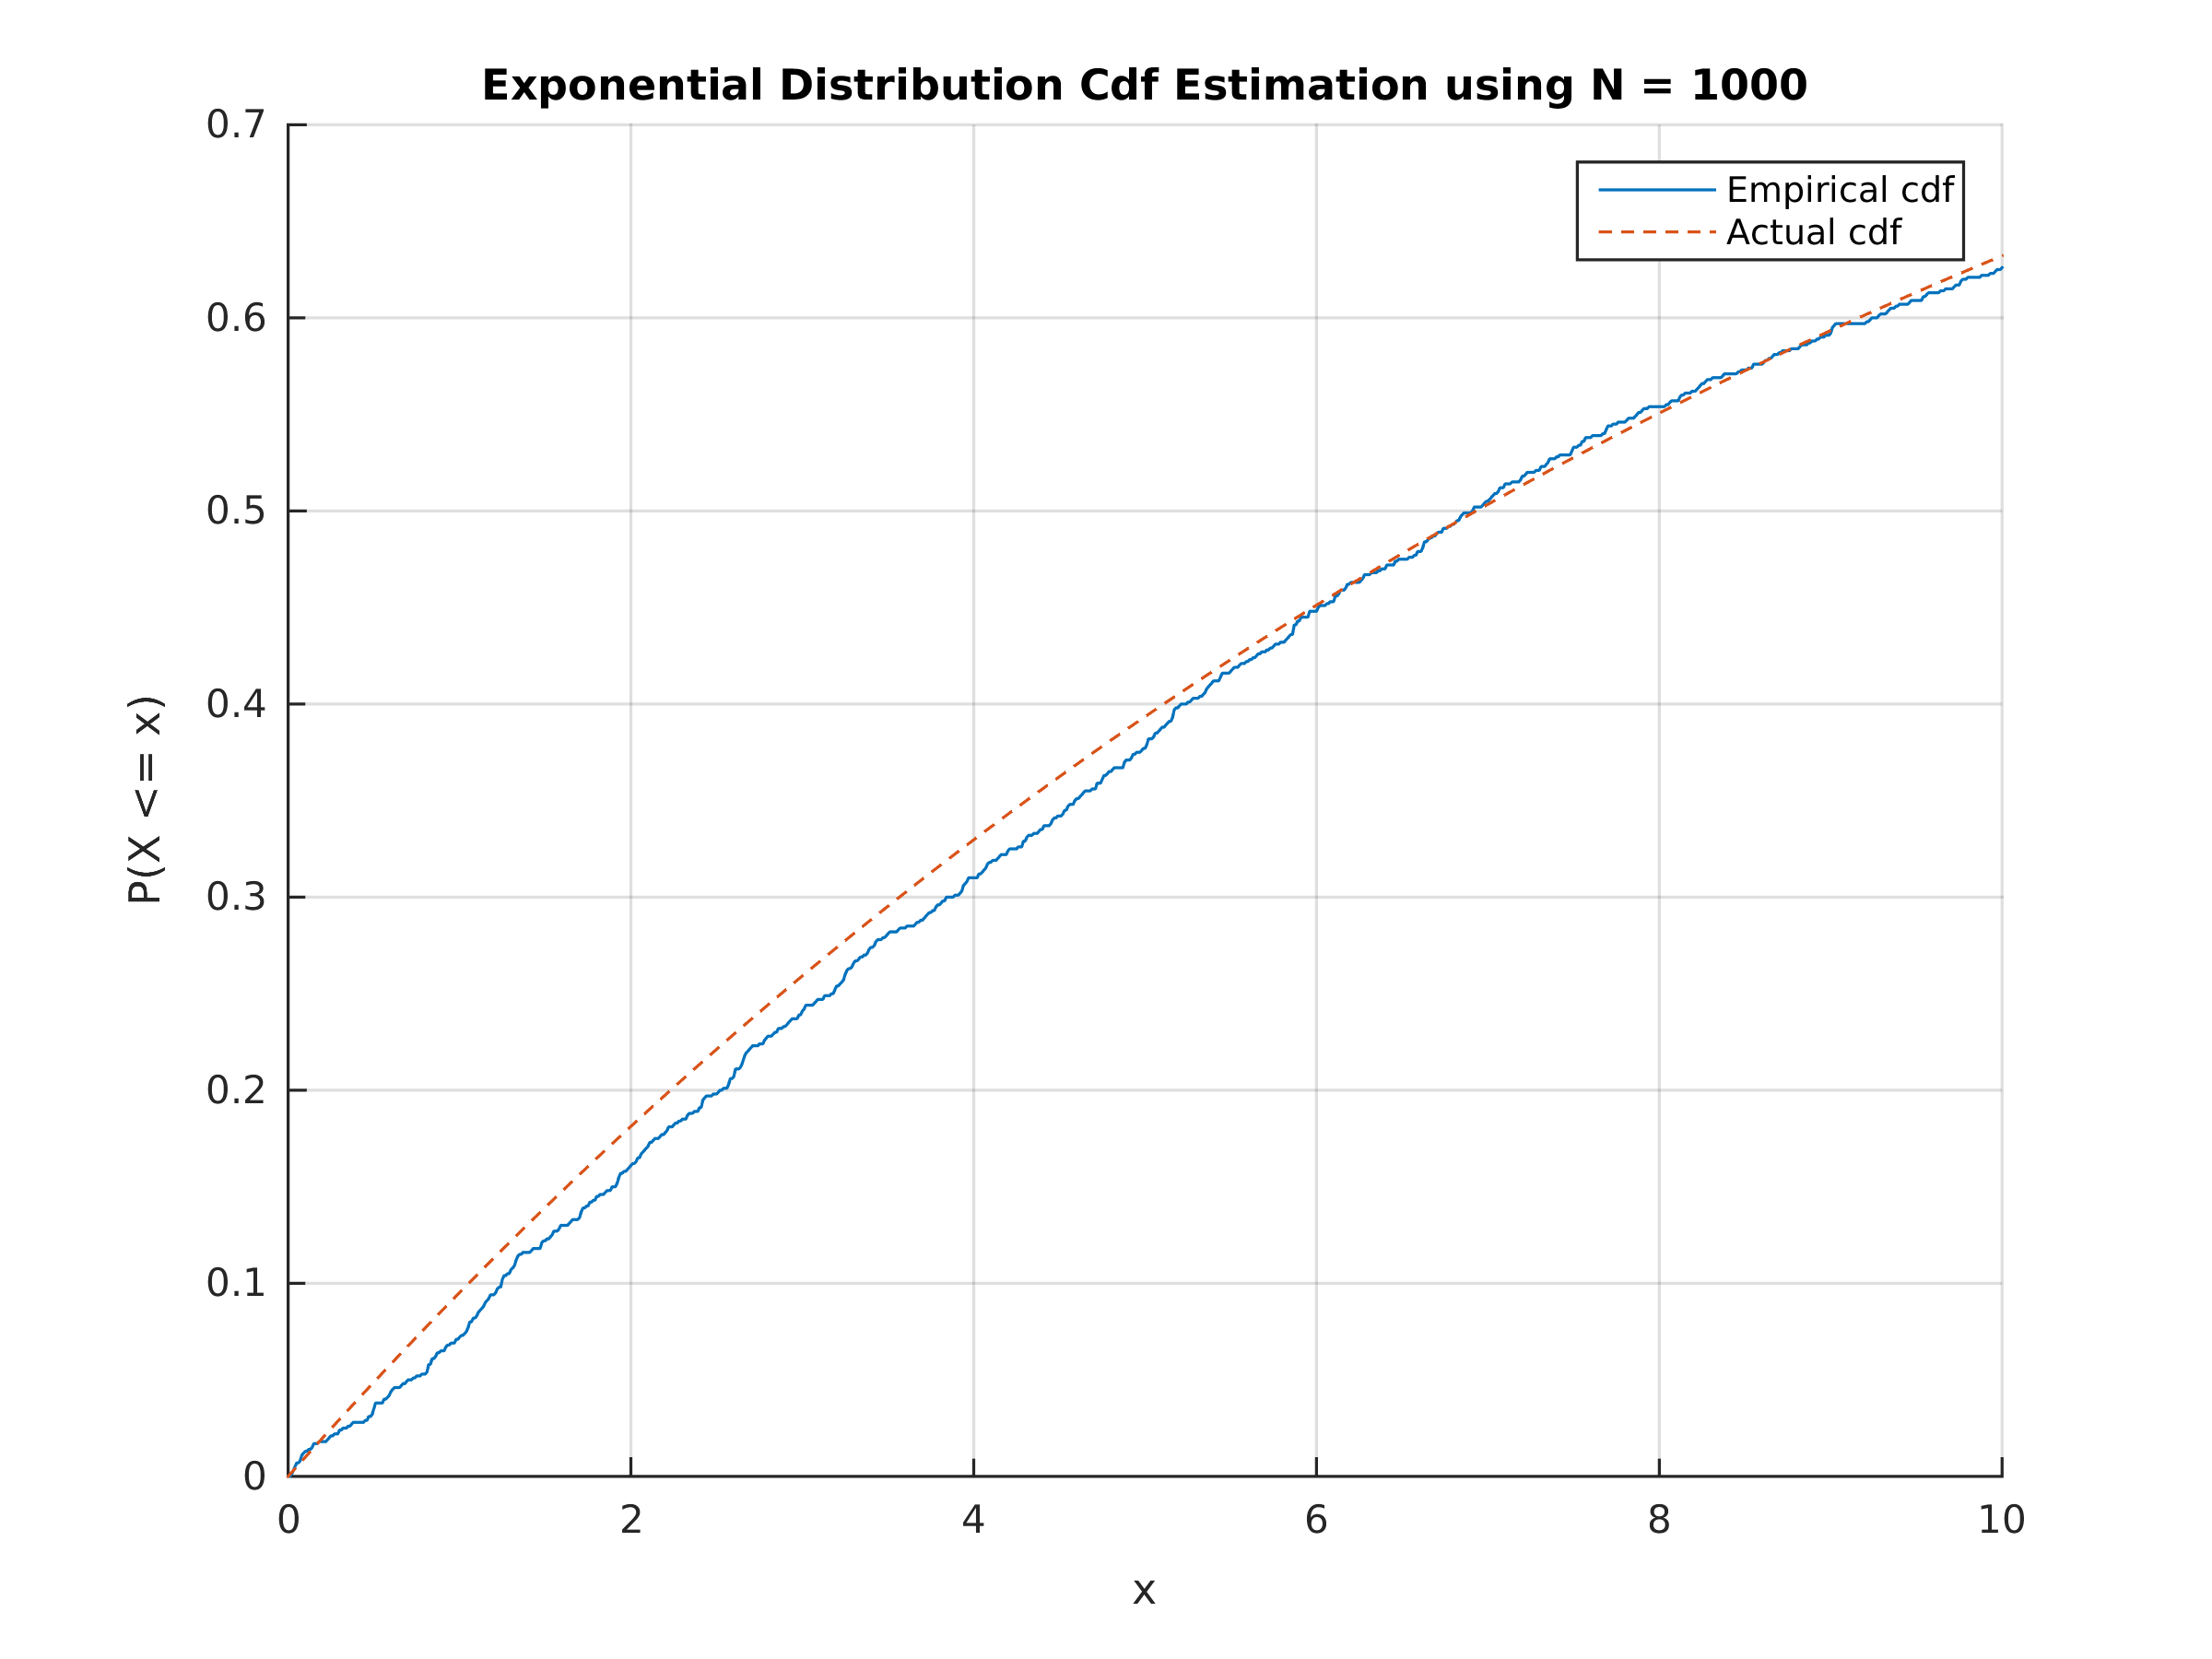
\includegraphics[width=1\linewidth]{hw2_8_exp_n1000.png}
				\caption{Cdf using $N = 1000$.}
			\end{subfigure}
			\caption{The cdf plots of poisson random variable $Y$.}
		\end{figure}
		When $N = 100$, the cdf follows the trend of the actual exponential
		distribution but does not fit entirely. When using 1000 samples, the cdf
		fits nicely. $E[X] = ???$.
	\subsection*{Problem 9}
	%TODO

\section*{MATLAB Code}
		\inputminted[tabsize=2,breaklines]{matlab}{hw2.m}

\end{document}
